\documentclass[multi,crop=false,class=article]{standalone}

\begin{document}
\section{Applications}
\label{sec:applications}


\subsection{Tools}
\label{ssec:tools}

In order to facilitate and promote active automata learning in a practical 
setting, tools have been created. This section will give a brief overview of
two tools. First, the tool Learnlib (\ref{sssec:learnlib}) will be discussed. 
This tool provide various active automata learning algorithms and 
optimizations. The second tool is Tomte(\ref{sssec:tomte}), which automatically 
generates abstractions for automatons in order to apply active automata 
learning on them. This selection is based on the importance of the tool, 
availability and the amount of researches that have used those tools.

\subsubsection{Learnlib}
\label{sssec:learnlib}

Learnlib  \footnote{Supported through bug fixes and available from 
\url{https://github.com/LearnLib/learnlib}} is a library that implements 
various active 
learning algorithms as well as different configurations for learning 
automata. It has been in development since 2009 \cite{Raffelt2009} and as of 
2015, there has been a total overhaul of the tool \cite{Isberner2015}. To avoid 
confusion, the old version was renamed to JLearn. 

The current version of this tool consists out of two parts: Automatalib and 
Learnlib.

\begin{figure}[!ht]
	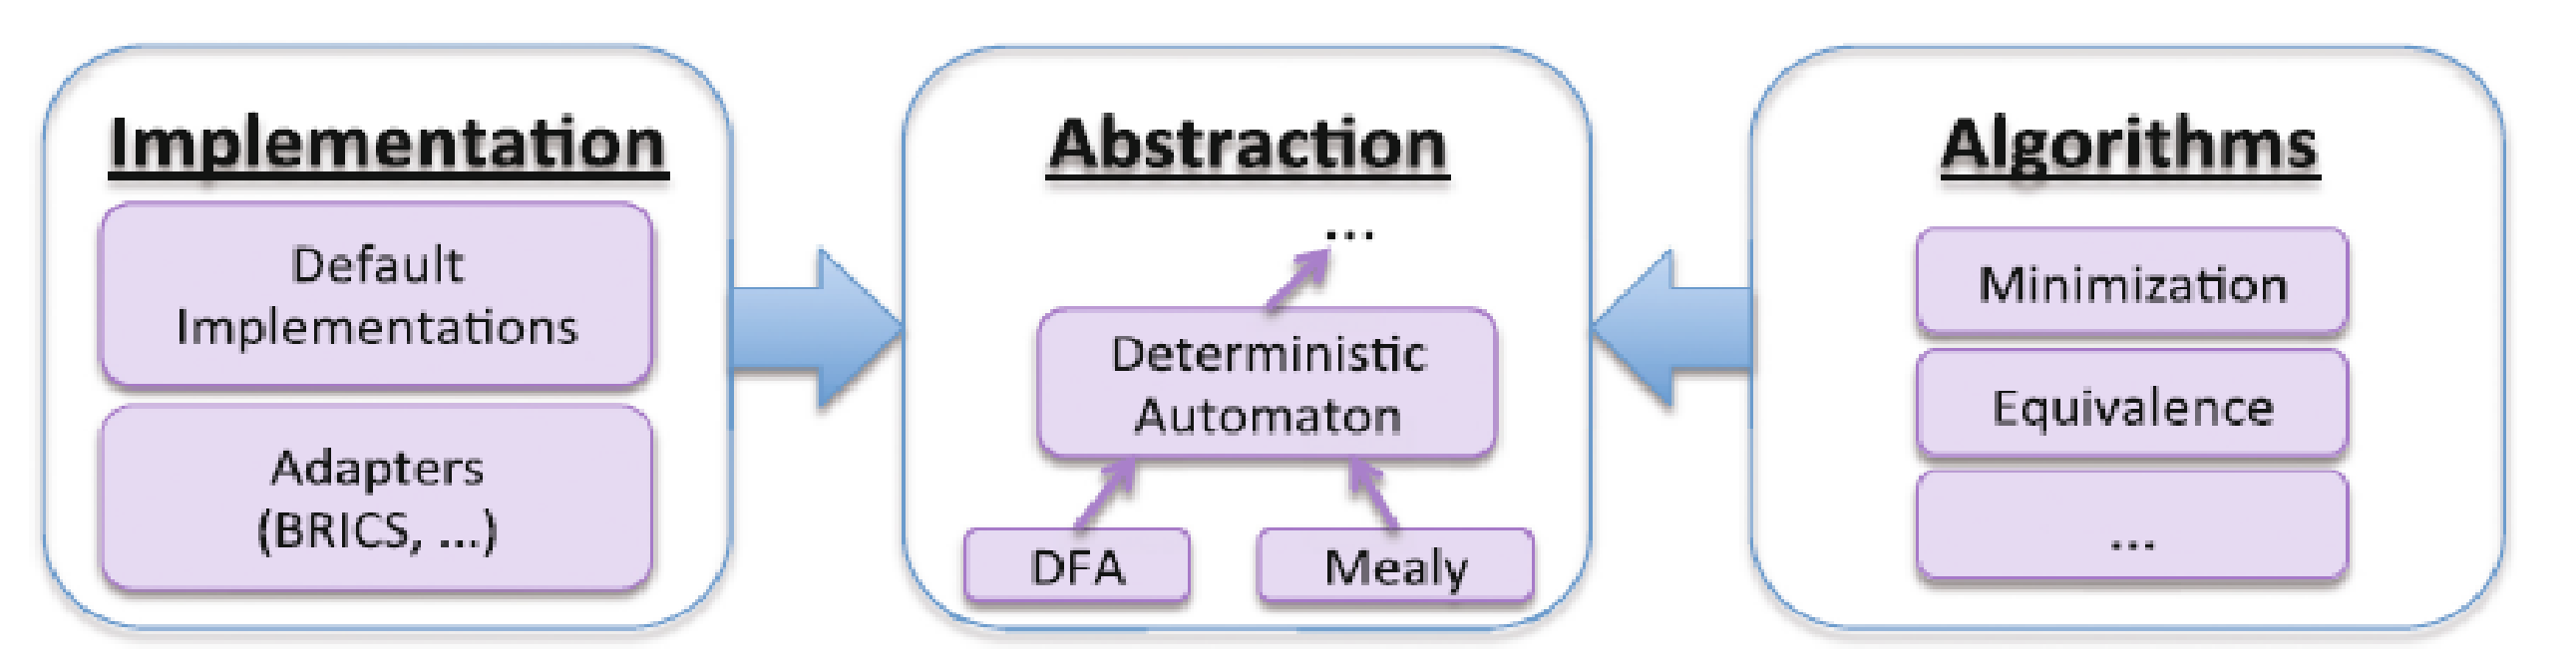
\includegraphics[width=\textwidth]{Tool_images/automatalib_architecture.png}
	\caption{Architecture of Automatalib, source is from \cite{Isberner2015}}
	\label{fig:automatalib_arch}
\end{figure}

\paragraph{Automatalib} An independent library that contains abstract 
automata representations, automata data structures and algorithms. The abstract 
automata representations make the library flexible because all data structures
and algorithms depend on those representations. This makes it easy to add 
third party implementations of automata like the BRICS library 
\cite{Alur2005}. Automatalib includes minimalization 
algorithms and equivalence testing algorithms based on Hopcroft and Karp's 
near-linear equivalence algorithm \cite{hopcroft1971} or the W-Method 
(X) \todo{Need a reference to the W-Method}  
for black-box testing. 

\begin{figure}[!ht]
	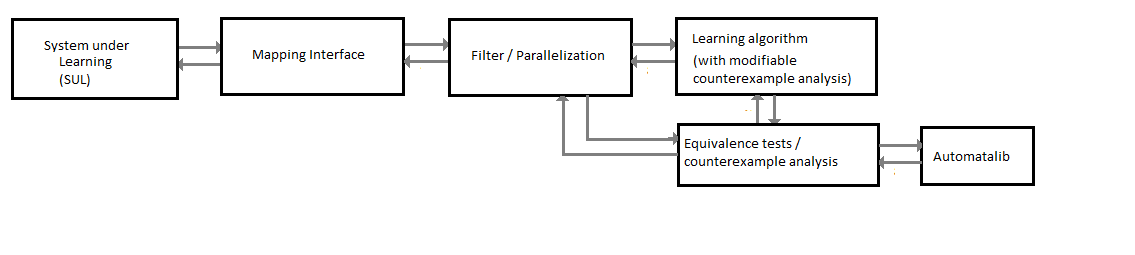
\includegraphics[width=\textwidth]{Tool_images/learnlib_architecture.png}
	\caption{Architecture of Learnlib}
	\label{fig:learnlib_arch}
\end{figure}

\paragraph{Learnlib} A library that provides learning algorithms and 
infrastructure for automata learning. The learning algorithms consist of a 
"base algorithm" whereby the counterexample analysis can be exchanged with 
other methods. All the different base algorithms with the examples of variants 
that are officially supported are listed below:

\begin{itemize}
	\item L* (base) (Explained in section \ref{sec:fundamental-theory})
	\begin{itemize}
		\item Maler \& Pnueli's \cite{Maler1995}
		\item Rivest \& Schapnire's (Summarized in 
		%\ref{sec:rivest-schap-count)) 
		\item Shahbaz's \cite{Shahbaz2009}
		\item Suffix1by1 \cite{irfan2010}
	\end{itemize}
	\item Obversation Pack (base) \cite{howar2012a}
	\item Kearns \& Vazirani's (base) (Summarized in 
	%\ref{sec:classification-trees)
	\item DHC (base) \cite{Merten2012}
	\item TTT (base) %\todo{Reference to theory does not exists, yet}
	\item NL* (base) \cite{Bollig2009}
\end{itemize}

All the algorithms come with both DFA and Mealy versions, expect for DHC and NL*.

For finding the counterexamples, Learnlib uses Automatalib as well as other 
methods like randomized tests. More methods can be found in \cite{Isberner2015}.

Learnlib also offers filters for reducing the amount of queries such as 
elimination of duplicate queries. %Is hier een theoriestuk over?
It also contains a parallellization component that can speed up the process by 
using multiple teachers and parallel execution of membership 
queries\cite{Henrix15}\cite{Howar2012}. 

\subsubsection{Tomte}
\label{sssec:tomte}
Tomte \footnote{In active development and available from 
\url{http://tomte.cs.ru.nl/Tomte-0-4}} is a tool that automatically makes 
abstractions for automata learning. Essentially, it a connector between the 
system under learning(SUL) and the learner. This makes using Learnlib and 
Libalf easier, since the user doesn't have to make the mapping.

\begin{figure}[!ht]
	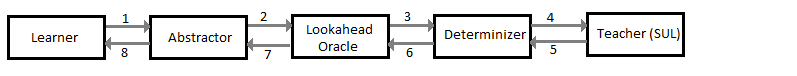
\includegraphics[width=\textwidth]{Tool_images/tomte_network.png}
	\caption{Architecture of Tomte}
	\label{fig:tomte_arch_interactoin}
\end{figure}

The Abstractor, Lookahead Oracle and the Determinizer together form Tomte. The 
other two parts are not part of Tomte but it comes with a supplied library 
(Learnlib) for making the learner.
The makers also have a tool \footnote{SUL Tool available from 
http://tomte.cs.ru.nl/Sut-0-4/Description} available for creating the SUL since 
they must be modeled after a register automata.
 
\paragraph{Determinizer}
The Determinizer elimates the nondeterministic behaviour caused by the SUL. 
Since tools like Learnlib can only analyse deterministic behaviour, it needs to 
converted. The theory behind it, is explained in \cite{Aarts2015}.

\paragraph{Lookahead Oracle}
This oracle is used to annotate events of the SUL with information about the 
impact on the future behaviour of the SUL. This way, the Looahead Oracle act as 
a cache for the Abstractor. The theory and implementation of 
this oracle is found in \cite{Aarts2014} and \cite{tomte14}.

\paragraph{Abstractor}
The Abstractor is the component that creates the mapping between the SUL and 
the learner. The idea behind the Abstractor is to make an abstraction of the 
parameter values of the SUL but leaving the input/output symbols unchanged. It 
uses counterexample-guided abstraction refinement\cite{tomte14} for extension 
of the mapping. In order to make it scalable, this component also tries to 
reduce the length of the counterexample by removing loops and single 
transitions \cite{Koopman2014}. The complete theory is found in \cite{tomte14}.

\paragraph{Interaction between the modules} The exchange of messages between 
all the modules is as follows(see numbering in figure 
\ref{fig:tomte_arch_interactoin}.
\begin{enumerate}
	\item Learner sends an abstract output query to the Abstractor.
	\item Abstracter receives an abstract query, selects a concrete input 
	symbol $i$ and send it as an output query to the Lookahead Oracle. If no 
	input symbol $i$ exists, return $\perp$ to the Learner.
	\item  Lookahead Oracle checks if $i$ is cached. If not, then $s$ is send 
	to the Determinizer. Otherwise, go to step 7.
	\item Determinizer transforms the input back to the original behavior of 
	the Teacher  
	\item Determinizer receives input from the Teacher and transforms this 
	nondeterministic behavior.
	\item Determinizer sends concrete symbol $o$ to the Lookahead Oracle which 
	caches input output pair $\{i,o\}$
	\item Lookahead oracle sends $o$ together with the annotated information 
	that came after the sequence of queries between the last reset query and 
	$i$.
	\item Abstractor receives a concrete answer $o$ and the annotated 
	information. It uses the annotated information to determine updates to the 
	state variables of the Learner. It sends those updates and other 
	information to the Learner as an abstract answer. 
\end{enumerate}


\end{document}

%%% Local Variables:
%%% mode: latex
%%% TeX-master: "main"
%%% End:
